\documentclass{article} % For LaTeX2e
\usepackage{nips13submit_e,times}
\usepackage{hyperref}
\usepackage{url}
\usepackage{amsmath, amsthm, amssymb, mathrsfs}
\usepackage{listings,courier,color}
\usepackage{tikz}
\usepackage[margin=1in]{geometry}
%\documentstyle[nips13submit_09,times,art10]{article} % For LaTeX 2.09


\lstset{language=Matlab}
\lstset{
	basicstyle=\footnotesize\ttfamily,
	breaklines=true,
	morekeywords={assert},
	showstringspaces=false
}
%% definitions.tex
%% @Diao Zheng

%% Contains definitions and shorthands for LaTeX template

% As of v2.2, the following are defined

%\+ : Logical conjunction
%\/ : Logical disjunction
%\! : Logical negation
%\afsoc : Assume for the sake of contradiction
%\amp : Ampersand
%\anf : Arbitrary and fixed
%\band : Conduction of indexed propositions
%\bb{} : Blackboard bold
%\bind{}{} : SML binding
%\bor : Disjunction of indexed propositions
%\ceil{} : Ceiling
%\circled : Circled text
%\code{} : Source code
%\codem{} : Source code in math mode
%\comb{}{} : Combination
%\cov{} : Covariance (matrix)
%\cp : Set compliment
%\D : Set of data
%\dash : Line
%\deriv{} : Derivative
%\derivn{}{} : Nth-order Derivative
%\eqnnum : Numbered equation
%\eqv : Equivalence
%\ev{} : Expected value
%\evc{}{} : Conditional expected value
%\F : False (Contradiction)
%\f : Fourier Transform
%\flr : Floor
%\fr : Fraktur
%\G : Script G
%\imp : Short implication symbol "=>"
%\inv : Inverse (of functions/matrices)
%\mat{} : Contained matrix
%\maxs{} : Maximum of a set
%\mins{} : Minimum of a set
%\mono{} : Monospaced text
%\N : Set of natural numbers
%\n : Set intersection
%\nil : Empty set
%\Nn : Set of natural numbers with zero
%\nn{}{} : Intersection of indexed sets
%\nullity : Nullity of a matrix
%\perm : Permutation
%\pderiv{} : Partial derivative
%\pderivn{}{} : Nth-order partial derivative
%\poly : Set of polynomials
%\prob : Probability
%\ps : Power set
%\R : Set of real numbers
%\rank : Rank of a matrix
%\Rn{} : Rn vector space
%\scr{} : Script
%\set{} : Set builder notation
%\summ{}{} : Summation
%\T : True (Tautology)
%\Tp : Topology
%\Tpb{} : Topology generated by a base
%\tx : Transformation
%\U : Set union
%\UU{}{} : Union of indexed sets
%\var{} : Variance
%\varc{}{} : Conditional variance
%\vc{} : Vector
%\x : Multiplication
%\Z : Set of integers










%augmented matrices
\makeatletter
\renewcommand*\env@matrix[1][*\c@MaxMatrixCols c]{%
  \hskip -\arraycolsep
  \let\@ifnextchar\new@ifnextchar
  \array{#1}}
\makeatother

\newcommand{\deriv}[1]{\frac{d}{d{#1}}}
\newcommand{\pderiv}[1]{\frac{\partial}{\partial {#1}}}
\newcommand{\derivn}[2]{\frac{d^{#2}}{d{#1}^{#2}}}
\newcommand{\pderivn}[2]{\frac{\partial^{#2}}{\partial{#1}^{#2}}}

\newcommand{\R}{\mathbb{R}}
\newcommand{\Rn}[1]{\mathbb{R}^{#1}}
\newcommand{\N}{\mathbb{N}}
\newcommand{\Nn}{\mathbb{N}_0}
\newcommand{\U}{\cup}
\newcommand{\n}{\cap}
\newcommand{\Z}{\mathbb{Z}}
\newcommand{\nil}{\varnothing}
\newcommand{\T}{\top}
\newcommand{\F}{\bot}
\newcommand{\eqv}{\Leftrightarrow}
\newcommand{\UU}[2]{\bigcup^{#2}_{#1}}
\newcommand{\nn}[2]{\bigcap^{#2}_{#1}}
\newcommand{\band}[2]{\bigwedge^{#2}_{#1}}
\newcommand{\bor}[2]{\bigvee^{#2}_{#1}}
\newcommand{\summ}[2]{\sum^{#2}_{#1}}
\newcommand{\poly}{\mathcal{p}}
\newcommand{\bb}{\mathbb}
\newcommand{\scr}{\mathcal}
\newcommand{\fr}{\mathfrak}
\newcommand{\ps}[1]{2^{#1}}
\newcommand{\cp}[1]{{#1}^C}
\newcommand{\f}{\fr{f}}
\newcommand{\amp}{\&}
\newcommand{\imp}{\Rightarrow}
\newcommand{\bmat}{\begin{bmatrix}}
\newcommand{\emat}{\end{bmatrix}}
\newcommand{\vc}{\mathbf}
\newcommand{\x}{\times}
\newcommand{\dash}{\rule[1mm]{10mm}{0.1pt}}
\newcommand{\circled}{\textcircled}
\newcommand{\eqnnum}
           {\stepcounter{eqnno}
             \dash\circled{\theeqnno}}
\newcommand{\+}{\wedge}
\renewcommand{\&}{\wedge}
\renewcommand{\/}{\vee}
\renewcommand{\!}{\neg}
\newcommand{\inv}[1]{{#1}^{-1}}
\newcommand{\tx}[1]{xrightarrow{#1}}
\newcommand{\Tp}{\scr{T}}
\newcommand{\set}[1]{\{#1\}}
\newcommand{\afsoc}{Assume for the sake of contradiction}
\newcommand{\anf}{arbitrary and fixed}
\newcommand{\Tpb}[1]{\Tp_{\scr{#1}}}
\newcommand{\maxs}[1]{\text{max }\{#1\}}
\newcommand{\mins}[1]{\text{min }\{#1\}}
\newcommand{\rank}{\text{rank}}
\newcommand{\nullity}{\text{nullity}}
\newcommand{\flr}[1]{\lfloor{#1}\rfloor}
\newcommand{\ceil}[1]{\lceil{#1}\rceil}
\newcommand{\code}[1]{\lstinline$#1$}
\newcommand{\codem}[1]{\text{\lstinline|#1|}}
\newcommand{\mono}[1]{\lstinline[keywordstyle={}]|#1|}
\newcommand{\bind}[2]{[\code{#1}/\code{#2}]}
\newcommand{\D}{\scr{D}}
\newcommand{\nCr}{\binom}
\newcommand{\perm}[2]{\,^{#1}P_{#2}}
\newcommand{\ev}[1]{\vc{E}[{#1}]}
\newcommand{\evc}[2]{\vc{E}_{#1}[{#2}]}
\newcommand{\var}[1]{\text{Var}[{#1}]}
\newcommand{\varc}[2]{\text{Var}_{#1}[{#2}]}
\newcommand{\cov}[1]{\vc{Cov}[{#1}]}
\newcommand{\prob}[1]{\vc{Pr}[{#1}]}
\newcommand{\comb}[2]{{{#1} \choose {#2}}}
\newcommand{\defeq}{\mathrel{\overset{\makebox[0pt]{\mbox{\normalfont\tiny\sffamily def}}}{=}}}



\title{10-601 Final Project Midway Report}


\author{
Simon Diao\\
Carnegie Mellon University\\
Pittsburgh, PA 15213 \\
\texttt{zdiao@andrew.cmu.edu} \\
\And
Nicolas Badoux \\
\'Ecole Polytechnique F\'ed\'erale de Lausanne \\
Switzerland \\
\texttt{nbadoux@andrew.cmu.edu} \\
}

% The \author macro works with any number of authors. There are two commands
% used to separate the names and addresses of multiple authors: \And and \AND.
%
% Using \And between authors leaves it to \LaTeX{} to determine where to break
% the lines. Using \AND forces a linebreak at that point. So, if \LaTeX{}
% puts 3 of 4 authors names on the first line, and the last on the second
% line, try using \AND instead of \And before the third author name.

\newcommand{\fix}{\marginpar{FIX}}
\newcommand{\new}{\marginpar{NEW}}

\nipsfinalcopy % Uncomment for camera-ready version

\begin{document}


\maketitle

\begin{abstract}
In this midway report, we managed to use a $k$th nearest neighbour classifier to achieve a reasonable classification accuracy of a subset of CIFAR-10 images dubbed \code{subset_CIFAR10}, albeit with slower runtime. We also implemented classifiers such as na\"ive Bayes and neural networks with little success. We have also investigated different features to use in classification.
\end{abstract}

\section{Introduction}

For this project, we aim to classify CIFAR-10 images dataset - a collection of 10000 32$\x$32 images, into one of ten categories, as per project requirements,
our classifiers are trained solely on a subset of 5000 CIFAR-10 images provided to us as \code{subset_CIFAR10}. As of this midway report, we have explored many
classifiers, including Na\"ive Bayes, logistic regression, neural network, deep neural network, convolutional neural network, and $k$th nearest neighbour. Due
to the complicated nature of neural networks, we have not yet found a set of satisfactory parameters that would give a decent output. However, we were able to
produce a $k$th nearest neighbour classifier with an accuracy of $53\%$\footnote{This classifier ran for 194 seconds on a local machine with a 2.4 GHz quad-core
processor. The classifier was highly parallelised, utilising \code{parfor} with 4 worker threads. The 53\% accuracy was tested on \code{test_batch.mat} from 
CIFAR-10 dataset.}

\subsection{Motivation}

We decided to focus primarily on neural networks due to its ability to model many abstract concepts, and neural networks, especially convolution neural networks (CNN), such as LeNet,
has seen great success in the area of image recognition. Our goal for this project is to implement a working CNN to classify the given dataset. However, in doing so, we would have 
to face many challenges, including initialisation of values, performing back-propagation on convolutional and pooling layers, and find the optimal set of parameters for optimal
performance.

\subsection{Background and Related Work}

Xavier Glorot and Yoshua Bengio [1] noted that initialisation of neural network weights should be sampled from a distribution of mean 0 and variance $\frac{2}{n_{in}+n_{out}}$.
Further research was done in attempt to understand convolutional neural networks in terms of concept and implementation. Heaton noted that the following was to be considered when determining the size of hidden layers in a neural network [2]:
\begin{itemize}
  \item The number of hidden neurons should be between the size of the input layer and the size of the output layer.
  \item The number of hidden neurons should be 2/3 the size of the input layer, plus the size of the output layer.
  \item The number of hidden neurons should be less than twice the size of the input layer.
\end{itemize}



\section{Method}
Methodology is further broken down into three parts, classifiers, feature selection and training.

\subsection{Classifiers}
We have attempted and tried various supervised learning algorithms, some with more success than others.

\subsubsection{Na\"ive Bayes}
The Na\"ive Bayes classifier seeks to maximise
$$\prob{Y|X}$$
with the assumption that
$$\forall i,j,  i\neq j \cdot \prob{X_i|X_j, Y}=\prob{X_i|Y}$$
In other words, it assumes that all input features are conditionally independent of each other given the prior. However, in the case of image classification, this assumption does
not hold very well, as in a normal image, the intensity or colour of a pixel will depend on the intensities and colours of neighbouring pixels. Therefore, using raw pixel values (both 
RGB and HSV\footnote{Hue, Saturation and Value. This colour space separates the hue, or colour from its intensity and brightness, and we can treat the three values as essentially independent of each other.}), we were only able to achieve around $30\%$ classification accuracy. Using histogram of oriented gradients improved the classification accuracy to $48.7\%$. However, we
were unable to improve on the classification accuracy. We did attempt to change the \code{cell_size} parameter, however, we found that at higher values, it leads to overfitting, and
at lower levels, it reduces classification accuracy.

The classifier was implemented as Gaussian features each with a mean and variance estimate. Log likelihood was used to avoid floating-point underflow. However, other posterior distributions could also be considered, such as Beta in case of pixel values.

\subsubsection{Neural Network}
Most of our time was focused on attempting to produce a useable classifier using a neural network. We implemented three variants of neural networks, a simple neural network with 1 hidden layer, a deep neural network with multiple hidden layers of the same size, and a convolutional neural network with one convolutional layer, one pooling layer and a fully connected layer.

For all of our neural network layers (other than the convolutional and pooling layers), the activation function is given as

$$o = \frac{1}{1+e^{-X\cdot W}}$$

where $o$ is the output, and $X$ is the input layer and $W$ is the associated weight, which we then initialised using Xavier initialisation discussed earlier and trained using back-propagation.
We also used entropy as objective function, where
$$\delta_k = o_k(1-o_k)(t_k-o_k)$$
where $t_k$ is the expected output of the $k$th neuron. Furthermore, for all of our neural network implementations, the final layer had 10 neurons, each indicating a class probability. The final decision is reached by 
$$\arg\max_k o_k$$

In order to visualise the gradient descent, we implemented two error functions:
  $$E_1 = \summ{i}{}{|t_i-o_i|}$$
and
  $$E_2 = \summ{i}{}{(t_i-o_i)^2}$$
Both these errors were only used once per epoch to test for convergence, which we defined as $E_{t}\geq E_{t-1}$.

The final classifier we decided to implement consists of 496 input layers, each corresponding to a HOG feature (with a cell size of 8), 236 hidden layers and 10 output layers. The activation function for each of the hidden layers is as follows:
  $$o = \frac{1}{1+e^{-(x\cdot w+b)}}$$
where $w$ is the weight given to any of the $x$s, and $b$ is a scalar that indicate the bias of this neuron. Both $w$ and $b$ are learnt by stochastic gradient descent. with a learning rate $\eta=0.001$ and momentum $\alpha=0.8$.


\subsubsection{$k$th Nearest Neighbour}
Our final attempt at a classifier was to implement $k$th nearest neighbour with a image kernel. $k$th nearest neighbour seeks to find the, as the name suggest, $k$ nearest neighbours and obtain the mode label. We have tried a variety of input features with this algorithm, including dominant colour, scale-invariant feature transform (SIFT), and histogram of oriented gradients (HOG). For SIFT, the distance metric was to first perform \code{vl_ubcmatch} on test sample and neighbour, and order neighbours by number of matches and then by sum of distance, so suppose that
\begin{lstlisting}
  [~, scores] = vl_ubcmatch(sample, neighbour);
  [n, d] = size(scores);
\end{lstlisting}
then
$$A < B \eqv \codem{n}_A>\codem{n}_B \/ (\codem{n}_A=\codem{n}_B\+\summ{i=0}{\codem{n}_A}{\codem{scores}_{A,i}}<\summ{i=0}{\codem{n}_B}{\codem{scores}_{B,i}})$$

However, this metric did not perform very well, and its classification accuracy was around $30\%$.

We also used HOG features with $\codem{cell_size}=8$. Here, our distance metric is the L1 sum of the difference of the HOG features. Suppose that the HOG feature of each image is a $N\x N\x K$ tensor, and the HOG features of the test image and its neighbour is $F$ and $G$ respectively, then our distance metric can be characterised as
$$d=\summ{i=1}{N}\summ{j=1}{N}\summ{k=1}{K}|F_{ijk}-G_{ijk}|$$

This classifier is our best performing classifier so far, with an accuracy of $53\%$. Our final attempt also included the most dominant colour (in RGB) in the image.

Unfortunately, our only optimisation done so far for this classifier was to use \code{parfor} instead of \code{for} to invoke parallelism in code, and that has brought the runtime down to around 3 minutes on a multi-core machine using Matlab's Parallel Computing Toolkit. We are, however, aware that the Toolkit is not available in Octave, and we would not be utilise it during the final submission. Hence, we are also looking at other optimisations, such as implementing a $k$-d tree to hold the nearest neighbour.

\subsection{Features Extraction}
We have attempted to extract different features from the image in order to reduce noise in the data.

\subsubsection{Raw Pixel Data}
We have trained some classifier with the raw pixel value, both RGB, HSV and intensity. Until now we did not get a good result. However, we are hopeful that a well-trained convolutional neural network would be able to produce reasonable results with raw pixel values.

\subsubsection{Dominant Colour}
We noticed that some colours in the image only appears on specific classes, such as red, thus we theorised that dominant colours could aid us in classification. To obtain it, we applied a blur to the image to smooth the colour. To extract the dominant color, we sampled the image every 4 pixels and compared the colour sampled to every pixel in the image, counting how many pixels are in a certain range of the sampled color.

We sample every four pixels to spare some computations. Since we are trying to find the dominant colour, it's quite certain that even looking to only one fourth of the pixel we will encounter the most dominant colour. We also check that the colour picked is not the already dominant colour. The range is 100 and is the sum of the differences between the R, G and B values. 

\subsubsection{Edge detection}
We apply a simple Sobel algorithm on the grayscale image. We have also implemented an edge detection on the different R, G and B channels and then regroup the different edges. This give us an interesting result, some edges appear only in some color channel (like between a blue sky and a blue sea, the blue channel would not give us any result but the red channel can). Comparing it with the grayscale edge detection give also some feedback.

\subsubsection{Horizontal Line}

We also tried to find an horizontal edge in the image. This could mean an horizon (like in the case of a ship at sea) or a straight horizontal line (for example a photo of a truck sideways). To extract this feature, we first applied the Sobel algorithm to the image with reasonable threshold (0.14 in this case). Then we went trough the lines of the image and counted how many pixel were on the line, just above or just below and are marked as edges. A higher number represent lot of edges in the same horizontal area. 

To counter the case were we would just had a lot of edges but not specially in a horizontal shape and not give a higher score with an image with fewer pixel marked as edges but all in an horizontal line, we subtract to the highest number we found, the 4th highest number. That means, we take the group of 3 lines with the maximum of pixel denoted as edges and decrease this value by the number of pixel denoted as edges in another group of 3 lines. Therefore, if the image has lot of pixel marked as edges but not particularly in a horizontal line, the score would be much nearer to zero. 

\subsubsection{Histogram of Oriented Gradients}
We have also used VLFeat to extract the Histogram of oriented gradients (HOG).
We are still trying to adjust the cell size to match at best our classifier without timing out. 
The HOG values give us some insight on the edges as well as on color or intensity value of the image. Therefore it's a quite interesting feature that gave us some good result alone. 

\subsection{Training}
We have also attempted various methods of training the different classifiers. For Na\"ive Bayes, we used MLE log likelihood with Gaussian likelihoods. However, if we were to use feature values that which are bounded in one end or two, other distributions, such as Gamma or Beta could prove to be more useful. We could also use semi-supervised learning and boosting to boost the performance of Na\"ive Bayes classifier.

For the neural networks, we were using stochastic gradient descent with batch sizes of 5000. We added a momentum factor as our classifier was often getting stuck at local optima - it found a minima where it gives the same classification to all images, and could not move past that point. There is obviously much to learn and research about neural networks.

For $k$th nearest neighbour, we would need to store the neighbours in a more organised data structure instead of a list. The current $k$NN algorithm we have runs in $O(nd)$ work and $O(d)$ span, where $n$ is the number of test samples and $d$ is the number of training samples. However, with the implementation of a $k$-d tree data structure, we could lower the work and span bounds to $O(n\log d)$ and $O(\log d)$ respectively.

\section{Experiments and Results}

\subsection{Selection of Hidden Units in Neural Network}

Our neural network classifier design used 496 input neurons as the result of a HOG feature with cell size 8, and 10 output neurons each representing the probability of classifying the image into one of the classes. The class picked is the class label with the highest probability, i.e. $\arg\max_i {x_i}$. To determine the optimal number of neurons in the hidden layer, we conformed to Heaton's suggestions [2] and trained 3 neural networks each with a number of hidden neurons ranging from 200 to 300, resulting in 300 different networks. Each of the networks is trained with a learning rate $\eta=0.001$ and momentum $\alpha=0.8$. For each network, we computed the training accuracy and test accuracy. Training accuracy was achieved by running the classifier on the 5000 given training samples, whereas test accuracy was achieved using the 10000-image \code{test_batch} in the CIFAR-10 dataset. We then plotted the $\max$ of both training and test accuracy\footnote{The classifiers with the $\max$ training and test accuracies are not necessarily the same ones.}. The results are shown in Figure 1. We have seen that the test accuracy is relatively consistent when the number of hidden neurons is between 200 to 260, however, as the number of neurons increases above 290, the chances for gradient descent to find a local minimum that is giving a baseline reading of 0.1\footnote{This baseline is simply classifying everything as one class (i.e. picking the most popular class label).} increases. However, it could also be that we are extremely unlucky in our simulation where none of the 3 initialisations gives the optimal result. running Matlab's \code{max} function on test accuracy gives the number of hidden neurons to be 236, which is the value we used as hidden layer. We noticed that for non-baseline classifiers, the training accuracy is significantly higher than test accuracy, and the training accuracy also fluctuates much greater than test accuracy. Hence, we conclude that a hidden layer of anywhere between 200-260 neurons could be optimal for our network.

\begin{figure}
\centering
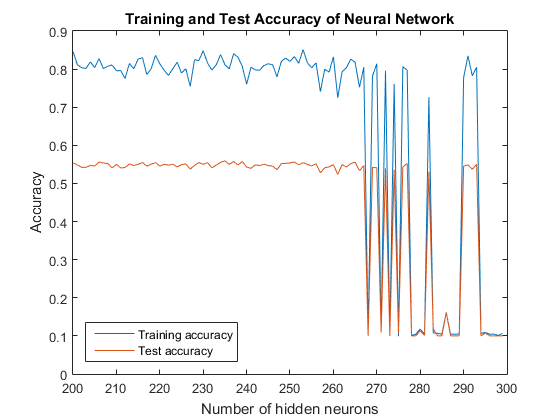
\includegraphics{fig1.png}
\caption{The training and test errors for our neural network.}
\end{figure}




\section{Conclusion and Further Improvements}
We will continue to improve our features extraction and make it match at best with our different classifiers. This can for example mean finding the good threshold for the edge detection or change the linearity of the score of the horizontal line feature. Our plans also include to try different combinations of features to get the best result without compromising some classifiers assumptions (like Na\"ive Bayes assumptions).

We will try to use Scale-invariant feature transform (SIFT) to gain other insights into the image. In addition, we feel that a support-vector machine using SIFT as feature could yield a fairly decent classifier, and we would investigate into SVMs more.

We would also like to learn and complete the implementation of neural networks, especially CNNs, and implement a effecient and fast back-propagation algorithm for the learning of these networks. We would also want to optimise the factors, such as filter size, pooling size, and number of convolutional layers, pooling layers and hidden layers in the fully connected stage, as well as learning parameters such as $\eta$ and $\alpha$. We would also like to investigate into how to implement and learn the bias related to convolutional layers and sigmoid layers.

Lastly, we would like to optimise $k$NN to utilise more effecient data structures.



\section{References}
\small{
Glorot, X., \& Bengio, Y. (2010). Understanding the difficulty of training deep feedforward neural networks. \textit{In International conference on artificial intelligence and statistics} (pp. 249-256).

Heaton, J. (2008). \textit{Introduction to Neural Networks for Java} (2nd ed., pp. 158-159). St. Louis, Mo.: Heaton research.
}

\end{document}
